\begin{frame}{X-ray photoelectron spectroscopy}
    \begin{columns}

    \column[T]{0.35\textwidth}

    \begin{figure}
        \centering
        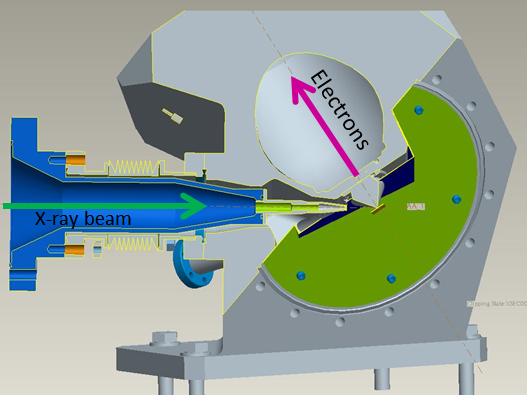
\includegraphics[width=0.7\textwidth]{Figures/xps_data/b07.png}
        \caption{B07-C branchline: Ambient Pressure XPS End Station (AP-XPS)}
        \label{fig:b07}
    \end{figure}

    \vspace{-0.5cm}
    \begin{table}
        \centering
        \begin{tabular}{ |l|l|l| }
            \hline
            Argon & \ammonia & \dioxygen \\
            \hline
            \rowcolor{lightblue}
            10 & 0 & 0 \\
            \rowcolor{lightorange}
            0 & 0 & 8.8 \\
            \rowcolor{lightgreen}
            0 & 1.1 & 8.8 \\
            \rowcolor{lightred}
            0 & 1.1 & 0.55 \\
            \rowcolor{lightviolet}
            0 & 1.1 & 0 \\
            \rowcolor{lightbrown}
            10 & 0 & 0 \\
            \rowcolor{lightpink}
            0 & 0 & 0.55 \\
            \hline
        \end{tabular}
        \caption{Partial pressures in reactor (mbar), in experimental order.}
    \end{table}
    
    \column[T]{0.63\textwidth}

    \begin{figure}
        \centering
        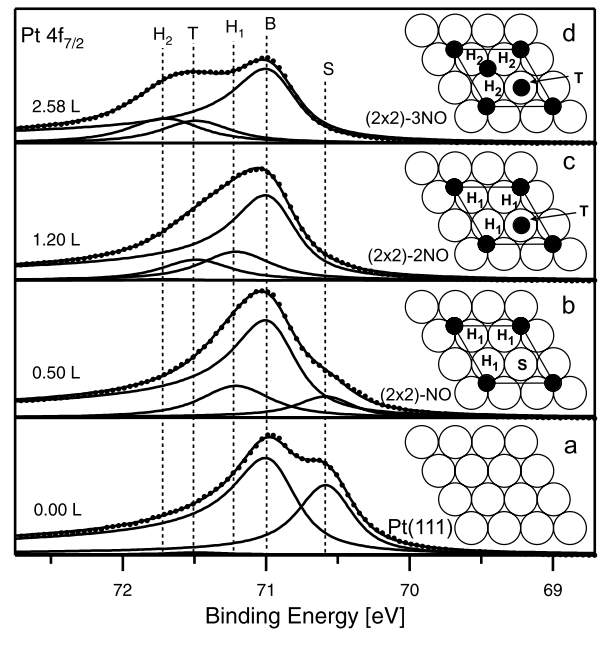
\includegraphics[width=0.6\textwidth]{Figures/xps_data/xps_multiple_peaks.png}
        \caption{Different components in the XPS spectra are linked to the coverage of the adsorbed species\footnotemark{}.}
        \label{fig:xps_multiple_peaks}
    \end{figure}

    \vspace{-0.3cm}

    \footnotetext{Zhu, J. F., Kinne, M., Fuhrmann, T., Denecke, R., Steinrück, H. P. (2003). In situ high-resolution XPS studies on adsorption of NO on Pt(1 1 1).Surface Science, 529(3), 384–396.}

    \end{columns}
    
    
\end{frame}